\section{The Gaussian chain: diffusion breaks locality}
\label{sec:gaussian}

\begin{figure*}[t]
  \centering
  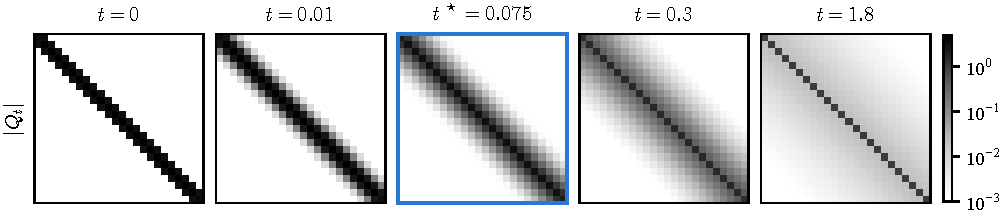
\includegraphics{fig_locality}
  \caption{Diffusion makes the score non-local. Magnitude of the score matrix $Q_t$ of the Gaussian chain
  ($\alpha=0.85$, $L=24$) at five noise levels, log colour scale. At $t=0$ it is the tridiagonal precision of the
  chain; at large $t$ it tends to the identity; in between, at $t^\star\simeq0.075$ (framed), the coupling beyond
  nearest neighbours is largest.}
  \label{fig:locality}
  % src: closed form, tools/paper_figs/make_paper_figures.py::fig_locality (t* = 0.0753 printed by the generator)
\end{figure*}

For the Gaussian chain everything is linear. The noisy data are Gaussian with covariance
$\Sigma_t=e^{-2t}\Sigma_0+\Dt\,I$, and the score is $S_t(x)=-Q_tx$ with $Q_t=\Sigma_t^{-1}$. At $t=0$ the matrix
$Q_0=\Sigma_0^{-1}$ is tridiagonal: this is the Markov property, written as a statement about the score. Each site
only talks to its two neighbours.

Diffusion does not preserve this. $\Sigma_t$ is a dense matrix plus a diagonal, and its inverse is not banded
(\cref{fig:locality}). The coupling of site $k$ to site $k+r$ decays geometrically in $r$, with a rate that depends on
$t$, and the matrix is furthest from tridiagonal at an intermediate level $t^\star\simeq0.075$ for $\alpha=0.85$
(\cref{app:numerics}). At large $t$ the noise dominates and $Q_t$ approaches the identity.
% src: t* = 0.0753, fig_locality / fig_locality_curve

The consequence is that locality cannot be obtained by constraining the denoiser. A denoiser that only sees a window
of radius $r$ around each site has an error floor even with unlimited data. For the Gaussian chain this floor is a
closed form: the best radius-$r$ estimator has relative score error $0.20$ for $r=1$, the nearest neighbours a
tridiagonal fit would use, $0.089$ for $r=2$, and still $0.029$ for $r=4$.
% src: thesis tools/fig_ch10.py::windowed_oracle([1,2,4,8]) = 0.2023, 0.0890, 0.0294, 0.0066 (alpha=0.85, L=32, 12 levels)
The structure has to be imposed elsewhere.

It is imposed on the model of the data. The posterior $p(a\mid x)$ is proportional to
$p_0(a)\prod_k\ell_t(x_k\mid a_k)$, with $\ell_t(x_k\mid a_k)=\Normal(x_k;e^{-t}a_k,\Dt)$, and is again a chain: the
noise is independent from site to site, so it adds one factor per site and no new link. For the Gaussian chain,
inference on this chain is the Kalman smoother \cite{kalman1960new,rauch1965maximum}, which returns $-Q_tx$ exactly
in $O(L)$ operations without ever forming $Q_t$. The next section does the same for any kernel.
